\section{RabbitMQ}

RabbitMQ merupakan salah satu message broker yang engimplementasikan model penyimpanan berbasis antrean dan mendukung persistensi pesan baik secara persisten maupun tidak kekal. Dari segi performa, RabbitMQ memiliki throughput hingga 60 ribu pesan per detik dengan latensi tergolong rendah (dalam milidetik). Model konsumennya bersifat \textit{push-based}, artinya broker secara aktif mengirimkan pesan ke konsumen. Alur ini ditunjukkan pada gambar \ref{fig:rabbitmq-flow}. RabbitMQ mendukung berbagai protokol seperti AMQP, MQTT, dan STOMP. Jaminan urutan pengiriman pesan pada RabbitMQ berlaku pada level antrean \parencite{arshadChoosingTheRightMessaging}.

\begin{figure}[htbp]
    \centering
    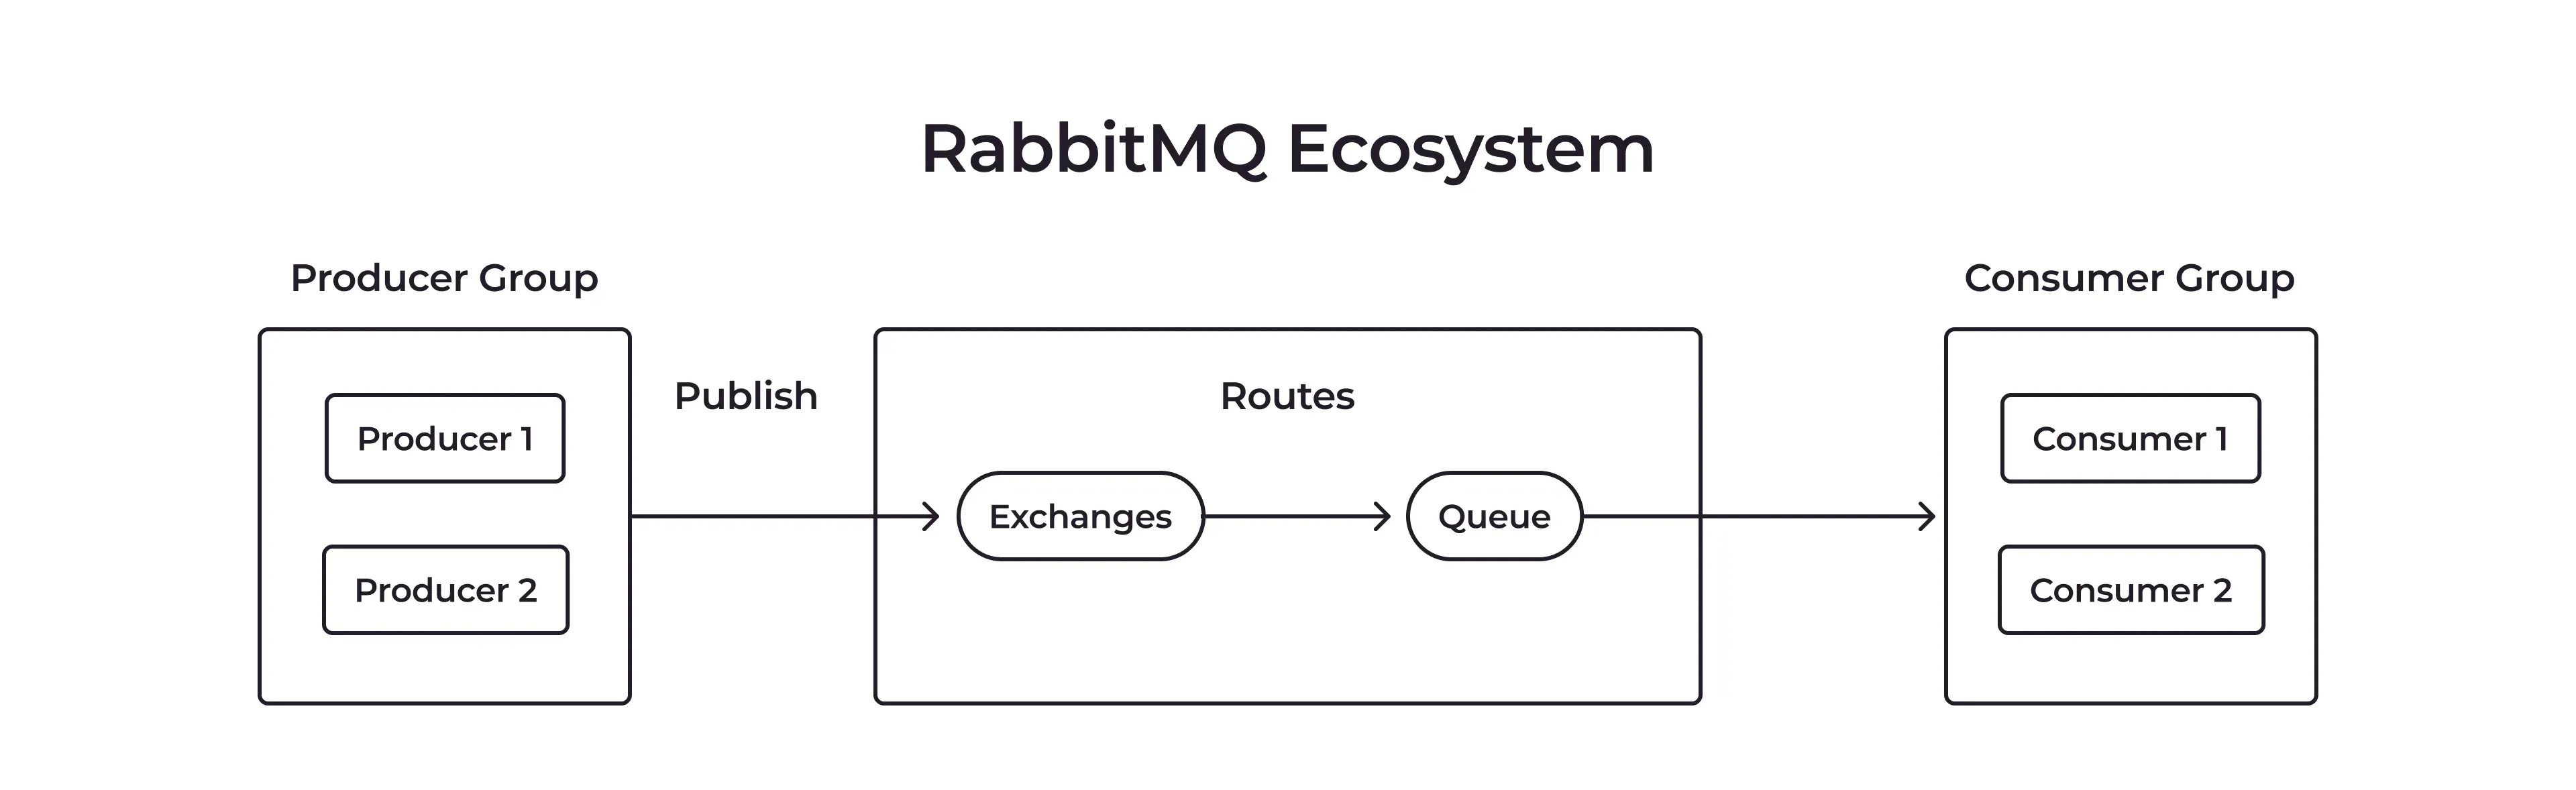
\includegraphics[width=0.8\textwidth]{resources/chapter-2/rabbitmq.jpeg}
    \caption{Alur RabbitMQ \parencite{royNatsRmqKafka}}
    \label{fig:rabbitmq-flow}
\end{figure}
